\documentclass{article}

% Language setting
% Replace `english' with e.g. `spanish' to change the document language
\usepackage[english]{babel}

% Set page size and margins
% Replace `letterpaper' with `a4paper' for UK/EU standard size
\usepackage[letterpaper,top=2cm,bottom=2cm,left=3cm,right=3cm,marginparwidth=1.75cm]{geometry}
\usepackage{CJKutf8}
% Useful packages
\usepackage{amsmath}
\usepackage{graphicx}
\usepackage{setspace}
\usepackage{float}
\usepackage{subfigure}
\usepackage{array}
\usepackage[section]{placeins}
\usepackage[colorlinks=true, allcolors=blue]{hyperref}
\usepackage[export]{adjustbox}

\author{B10209040 陳彥倫}

\begin{document}
\thispagestyle{empty}
\hfill {\scshape \large Cloud Physics, Fall 2023 } \hfill {\scshape P1}
\smallskip
\hrule
\begin{CJK*}{UTF8}{bsmi}
\bigskip
\bigskip
\bigskip

\centerline{\huge \textbf {HW4}}
\bigskip
\centerline{\textbf {B10209040 陳彥倫}}

\section*{1. Radar}

\subsection*{(1)}
    \begin{large}
        Plot results:
        \begin{figure}[!htbp]
            \centering
            \subfigure[i = -3]{
            \begin{minipage}[t]{0.5\linewidth}
            \centering
            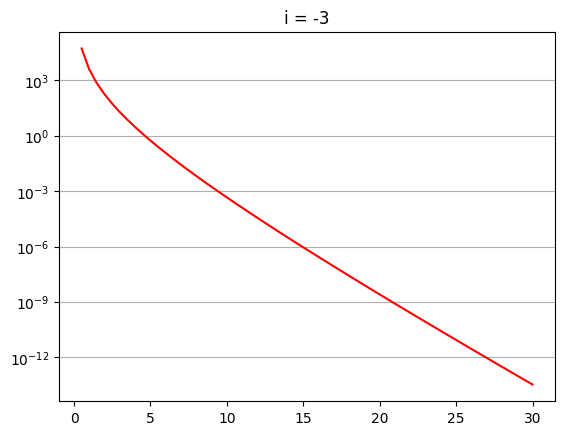
\includegraphics[scale=0.4]{output.png}
            %\caption{fig1}
            \end{minipage}%
            }%
            \subfigure[i = 0]{
            \begin{minipage}[t]{0.5\linewidth}
            \centering
            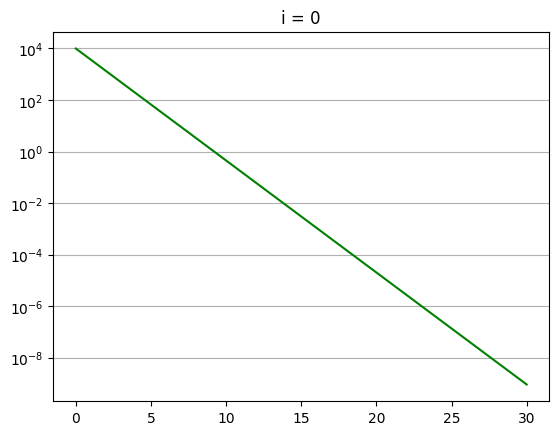
\includegraphics[scale=0.4]{output2.png}
            %\caption{fig2}
            \end{minipage}%
            }%

            \subfigure[i = 3]{
            \begin{minipage}[t]{0.5\linewidth}
            \centering
            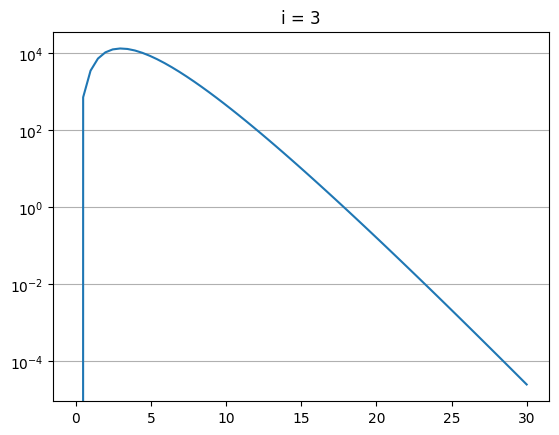
\includegraphics[scale=0.4]{output3.png}
            %\caption{fig2}
            \end{minipage}%
            }%
        \end{figure}
    \end{large}

\subsection*{(2)}
    \begin{large}
        \begin{center}
            \begin{displaymath}
                Z \equiv \sum\limits_{V}D^6 = \int_{0}^{\infty} D^6n(D) \,dD = \int_{0}^{\infty} D^6 \cdot N_0 \cdot D^i \cdot exp(-\lambda D^j) \,dD
            \end{displaymath}
        \end{center}

        \bigskip

        若$i = -3$時,將上述式子積分可得解析解:
            \begin{displaymath}
                Z = -10^4(D^3 + 3D^2 + 6D + 6)e^{-D}\bigg|^{\infty}_{0} = \mathbf{6 \times 10^4}\; mm^6/m^3
            \end{displaymath}

        \end{large}
        \newpage

\thispagestyle{empty}
\hfill {\scshape \large Cloud Physics, Fall 2023 } \hfill {\scshape P2}
\smallskip
\hrule
\bigskip
\bigskip
\bigskip
    
    \begin{large}
        若$i = 0$:
        \begin{displaymath}
            Z = -10^4(D^6 + 6D^5 + 30D^4 + 120D^3 + 360D^2 + 720D +720)e^{-D}\bigg|^{\infty}_{0} = \mathbf{7.2 \times 10^6}\; mm^6/m^3
        \end{displaymath}

        若$i = 3$:
        \begin{displaymath}
            Z = -10^4(D^9 + 9D^8 + 72D^7 + 504D^6 + \dots + 362880D + 362880)e^{-D}\bigg|^{\infty}_{0} = \mathbf{3.6288 \times 10^9}\; mm^6/m^3
        \end{displaymath}

    \end{large}

\bigskip

\subsection*{(3)}
    \begin{spacing}{3}
        \begin{large}
            \textbf{Discussion:} \\
                根據\;Modified gamma distribution fuction 及 \;standard gamma 的設定,並將\;y 軸調整成對數座標、
                x 軸設定為\;0$\sim$30\;mm,依序繪出\;i = -3, 0, 3 時的粒徑分佈。觀察三張圖可以看出粒徑分佈的主要變化是發生在
                \;D$<$10 處,i = -3 時為開口向上的曲線,但趨近於斜直線;i = 0 時則為斜直線。而\;i = 3 時則轉變為開口向下的曲
                線,且在粒徑約等於\;4 mm 時有數量分佈的最大值。\\
                另根據雷達回波因子之定義,積分計算各情況之值。發現隨著\;i 值的增加,Z 值也呈指數增加。
        \end{large}
    \end{spacing}




\end{CJK*}
\end{document}